\documentclass[conference]{IEEEtran}
\IEEEoverridecommandlockouts
% The preceding line is only needed to identify funding in the first footnote. If that is unneeded, please comment it out.
\usepackage{cite}
\usepackage{adjustbox}
\usepackage{amsmath,amssymb,amsfonts}
\usepackage{algorithmic}
\usepackage{graphicx}
\usepackage{textcomp}
\usepackage{xcolor}
\usepackage{hyperref}
\usepackage{tabularx}
\def\BibTeX{{\rm B\kern-.05em{\sc i\kern-.025em b}\kern-.08em
    T\kern-.1667em\lower.7ex\hbox{E}\kern-.125emX}}
\begin{document}
\title{\huge Metamorphic Testing in Cross-language Sentiment Analysis for Social Media}

\author{\IEEEauthorblockN{Boyang Yan}
\IEEEauthorblockA{\textit{School of Computing and Information Technology} \\
  \textit{University of Wollongong}\\
  Wollongong, Australia\\
  by932@uowmail.edu.au}
\and
\IEEEauthorblockN{Xiaoxia Pu}
\IEEEauthorblockA{\textit{School of Computing and Information Technology} \\
  \textit{University of Wollongong}\\
  Wollongong, Australia\\
  xp816@uowmail.edu.au
}
\and
\IEEEauthorblockN{Xudong Zhang}
\IEEEauthorblockA{\textit{School of Computing and Information Technology} \\
  \textit{University of Wollongong}\\
  Wollongong, Australia\\
  xz944@uowmail.edu.au}
\and
\IEEEauthorblockN{Helene Tran}
\IEEEauthorblockA{\textit{School of Computing and Information Technology} \\
  \textit{University of Wollongong}\\
  Wollongong, Australia\\
  ht185@uowmail.edu.au}
}

\maketitle

\begin{abstract}
  Huge amounts of text comments are posted on different topics in Social
  Media everday. These topics are discussed in different languages by different language
  speakers. Most people encounter language and culture barriers when engaging in
  cross-language communication. Cross-language opinion
  mining is useful for global integration. However, most research only focuses on
  English language sentiment analysis, but little research has been conducted on
  sentiment analysis in languages other than English. This research explores using machine
  trainslation and sentiment analysis tools to fill this gap. The research
  identifies a conbination of tools which will enable people to understand different language speakers' attitudes (positive or negative),
  emotions and opinions. This research is  based on the Metamorphic Testing method to establish a
  testing model for finding which machine translator service combined with which
  English sentiment analysis service can obtain reliable sentiment analysis
  results for non-English speakers who do not have sentiment analysis tools to
  analysis their own language. As a result, people will able to use Machine Translation
  and English Sentiment Analysis to conduct big data analysis in multi-language Social Media.
\end{abstract}

\begin{IEEEkeywords}
sentiment analysis, machine translation, Metamorphic Testing, Social Media,
Cross-Language, Cross-Culture
\end{IEEEkeywords}

\section{Introduction}

Social Media has been becoming more and more widely used. There are lots of text comments
on different discussion topics every day.
It would be impossible to analyses the huge amount of data generated manually.
These topics are discussed by speakers of different languages, from different
cultural backgrounds, further complicating any analysis.
Most people enounter language and cultureal barriers during cross-language
communication.
In this paper, the use of machine translation and sentiment analysis tools to
solve this problem of analysing cross-cultural and cross-language data is
explored and discussed.
Sentiment analysis is a part of text data mining. The aim of sentiment analysis
is to determine the attitude of speakers or writers with respect to particular topics
or the overall contextual polarity or emotional reaction to a text document. It is usually equated with
opinion mining, which involves the use of natural language processing and
machine learning to ascertain the possibility of positive or negative opinions \cite{sentimentAnalysis}.
Sentiment analysis is useful for analyzing a huge amount of data relating to personal
opinions. It can be used in an e-business context. For example, business managers can analysise
customers' attitudes, as to whether they like or dislike their product or service.
Also, government can use sentiment analysis to analyze citizen perspectives.
In a word, sentiment analysis is coming into widespread use.
As Dr. Haiyun mentions, English language sentiment analysis research has
undergone major developments in recent years \cite{ChineseSentimentAnalysis}.
However, less research has been undertaken in other languages, such as Chinese.
Today, a lot of English language sentiment analysis theories have been
developed. Also, a variety of Machine Translation tools is available, such as Google
translation, Bing translation and Yandex translation.
Manchine Translation uses computational linguistic programs and natural language
processing theory \cite{machineTranslation}.
However, nobody working in a combination of these two fields of research has undertaken non-English
sentiment analysis. Therefore, the research described and discussed in this paper aims to create a testing model to find the best-combination of English
sentiment analysis tools and machine translation tools to obtain reliable
sentiment analysis results from non-English texts, for non-English speakers who
do not have such sentiment analysis tools to analyze their own language.
Eventually, everyone will be able to understand different language speakers'
attitudes (positive or negative), emotions and opinions.\\
\section{Part A: Annotated bibliography}

\section{Literature Review}
This research consists of three components; measuring machine translation
service quality; testing sentiment analysis service quality;
finding the best compound mode for machine translation service and
sentiment analysis service.
As a result, this section will focus on a review of literature review about machine
translation, Testing methodology and sentiment analysis.
\subsection{Testing in Machine translation}
There are two research articles about testing modeling of machine
translation(MT).

\paragraph{Round Trip Translation method}
As Somers argues, an Around Trip Translation (RTT) method has been establish to
detect the quality of machine translation \cite{roundTripTranslation}; for example, testing English to Chinese translation tools.
Firstly, an English to Chinese translation tool is use to translate test data to
Chinese. It is then used to translate Chinese data back to English.
Finally, compare the similarity for two English data set.
They also mention two metrics of similarity, BLEU and F-score, to judge the
translations. The limitations of RTT model are it cannot distingicush the best
MT tool from a group of poor MT tools as well as it cannot find which sentences are easier for
translation and which sentences are harder for translation.

\paragraph{A Monte Carlo Method for machine translation services}
Another article is about using third-party language to test the quality of machine
translation \cite{thirdPartMachineTranslation}, for example, if testing an English to Chinese translation tool.
Firstly, random choose an Intermediate third-party language.
Secondly, translation English test data to the third-party language, after
translating, the third-party language to Chinese.
These two steps constitute one path.
Another path is translation from English directly to Chinese.
In the end, the two path results need to compare similarity. In this article, the main
finding is that Google Translate is the best machine translation compare with
Yandex, Youdao as well as Bing. In addition,
the better results to be produced in European languages compare with Asian languages, use ANOVA Statistics
method and Pairwise T tests giving this conclusion.
In my experiment, I also got Google Translator is the best machine translation
compare with Yandex and Baidu. Pairwise T tests also can be useful for finding best-combination of English
sentiment analysis tools and machine translation tools to obtain reliable
sentiment analysis results. The highlight of this model is using third-party
language, which can decide preference language of machine translation.

\subsection{Testing methodology}
Accounting to Sethi, there are two categorized testing
techniques, which are Static Testing and Dynamic Testing. The Dynamic Testing
are divided into three categories, which are Functional Testing, Structural
testing and Non-Functional Testing \cite{testingMethodReview}.
In my research project, I will focus on Functional Testing on this project.

\paragraph{Metamorphic Testing}
This research project is based on Metamorphic Testing.
Metamorphic Testing is for testing function correctness.
A research article written by Zhou in 2016 clearly explains what Metamorphic
Testing is.
As Zhou explains, Metamorphic Testing (MT) is a property-based software testing
method developed for automated test case generation and automated results
verification, based on the effects of some expected properties of the target
program \cite{zhou2016metamorphic}.
These properties, recognized as metamorphic relations (MRs), serve as essential
relations between the inputs and outcomes of multiple executions of the target
program.
For instance, calculator function correctness will be established if the input is 1 + 1,
and the result is 2. In this example people can easily make the judgment,
whether the calculator is functioning correctly or not.
However, people will not be able to easily make this judgment if the input is sin (3.7).
In a generally acknowledged, Sin (3.7) = sin (3.7 + 360) is correct.
In metamorphic testing, the name of 3.7 is the test case. The name of 3.7 + 360
is the follow-up test case.
Metamorphic Relation is the relationship between two input test cases as well as
the two outputs.
Metamorphic testing is based on Metamorphic Relation.
The two outputs need an existing mathematical relation.
In this example, the relation is “=”. However, MR does not must be an equation,
it also can be a relation.
The advantage of Metamorphic testing (MT) method; addressing the test oracle
problem; testing case generation problem.
The disadvantage is that it cannot detect memory leak or some others insensitivity
failure situation.
However, Metamorphic Testing is appropriate for testing translation tools and
sentiment analysis tools.
\paragraph{Effectiveness of Metamorphic Relations}
\cite{cao2013correlation}
There is another article which was written by Zhou about Effectiveness of
Metamorphic Relations in 2013.
The main purpose of reading this article is trying to find which Metamorphic
Relations can be the most efficient detecting failures.
Round Trip Translation and a Monte Carlo Method can be seen as two Metamorphic Relations.
This article is based on white-box testing, which have source code, as well as
the most important conclusion is if the Metamorphic Relations can get bigger
distance (dissimilarity) that will have more chance to detect failures.
In other words, MRs with very different initial and follow-up execution are more
likely to detect failures than those with similar initial and follow-up
executions.
The concept of ``difference'' are defined in namely coverage Manhattan distance
(CMD), frequency Manhattan distance (FMD), and frequency Hamming distance (FHD)
in regard to adaptive random testing (ART), where CMD metric on the basis of
branch coverage execution profiles performs the best fault-detection
effectiveness.
The advantage of this article is suitable for finding the most effectiveness of
Metamorphic Relations in White-box.
However, this article is not suitable for Black-Box Testing. The reason is
Black-Box Testing have not source code available, so it cannot calculate the
program’s distance.
In this research project, translation tools have NOT source code available, this
article is not suitable for this research accordingly.
\paragraph{White-box VS Black-box}
\cite{henard2016comparing}
There are another research article written by Henard in 2016. Talking about the difference between black-box testing and white-box testing.
Henard (2016) have done some research for difference between white box testing
and black - box testing in 2016. They have two finding is useful in my research
black-box testing and white-box testing performance just have a little
difference (at most 4 fault detection rate difference). They also found
black-box testing and white-box testing the overlap is
very high. The first 10 of the prioritized test data
already agree on at least 60 of the faults found. As the
result, this research article has given me a lot of ideas of how the similarity between white-box testing and black-box
testing. I still have opportunity for compare those three
modelings, which one is better.
\pagebreak
\pagebreak
\section{Research Proposal \protect\footnote{This research proposal is based on
    Boyang Yan's Master of Research application (research proposal section) in
    2017}}
\subsection{TITLE}
Metamorphic Testing in Cross-language Sentiment Analysis for Social Media
\subsection{Background and Research Problems}
Social Media has been becoming more and more widely used. There are lots of text comments
on different discussion topics every day.
It would be impossible to analyses the huge amount of data generated manually.
These topics are discussed by speakers of different languages, from different
cultural backgrounds, further complicating any analysis.
Most people enounter language and cultureal barriers during cross-language
communication.
In this research, the use of machine translation and sentiment analysis tools to
solve this problem of analysing cross-cultural and cross-language data is
explored and discussed.
Sentiment analysis is a part of text data mining. The aim of sentiment analysis
is to determine the attitude of speakers or writers with respect to particular topics
or the overall contextual polarity or emotional reaction to a text document. It is usually equated with
opinion mining, which involves the use of natural language processing and
machine learning to ascertain the possibility of positive or negative opinions
\cite{sentimentAnalysis}.
Sentiment analysis is useful for analyzing a huge amount of data relating to personal
opinions. It can be used in an e-business context. For example, business managers can analysise
customers' attitudes, as to whether they like or dislike their product or service.
Also, government can use sentiment analysis to analyze citizen perspectives.
In a word, sentiment analysis is coming into widespread use.
As Dr. Haiyun mentions, English language sentiment analysis research has
undergone major developments in recent years \cite{ChineseSentimentAnalysis}.
However, less research has been undertaken in other languages, such as Chinese.
Today, a lot of English language sentiment analysis theories have been
developed. Also, a variety of Machine Translation tools is available, such as Google
translation, Bing translation and Yandex translation.
Manchine Translation uses computational linguistic programs and natural language
processing theory \cite{machineTranslation}.
However, nobody working in a combination of these two fields of research has undertaken non-English
sentiment analysis. Therefore, the research described and discussed in this paper aims to create a testing model to find the best-combination of English
sentiment analysis tools and machine translation tools to obtain reliable
sentiment analysis results from non-English texts, for non-English speakers who
do not have such sentiment analysis tools to analyze their own language.
Eventually, everyone will be able to understand different language speakers'
attitudes (positive or negative), emotions and opinions.\\
The purpose of the study have two aspects.
The first aims of this research is to compare and analysis Google, Youdao, Baidu, Bing and
Yandex translation tools, which one is the best machine translation tool.
Second aim is creating a testing model to find the best-combination of English
sentiment analysis tools and machine translation tools to obtain reliable
sentiment analysis results.
Third aim is to create our own sentiment analysis model for
recognizing English data belonging to positive, negative, neutral or mix
classification. It is building by VADER, NLTK, LIWC, ANEW or the General Inquirer.
\subsection{Critical Review of Literature}

\subsection{Aims and Objectives}
The aim for this research is to achieve a method to find out the combination
between machine translation tools and English sentiment analysis model can
obtain the result, which is the most reliable and efficient, for those
non-English speakers, to fill the blank and gap of lacking of cross-language
sentiment analysis tool.
The main aim can be divided into 4 sub-aims.
\begin{enumerate}
  \item Advertisement Detection \\
Detect advertisements and junk contents among mass of data from social media
texts. Removing unimportant data can both reduce the amount of the size of whole
dataset to save processing time, and get rid of contents that is of no use to
our sentiment analysis, which can be also regarded as noise data.
  \item Data Preprocessing and Feature Extraction \\
Preprocessing data is to segment texts into words and select those words which
is helpful and sensitive in sentiment analysis. E.g. keywords, important
punctuation marks, emotion symbols. Also, normalization operations will be taken
to convert the keywords into it root form, which can reduce the size of lexicons
of models to a large extend. Then, extracting features of those data being
preprocessed as inputs for sentiment analysis model built by us.
  \item Sentiment Analysis Modelling \\
Develop a model for sentiment analysis which includes a lexicon placing emphasis on social media texts and a machine learning model for analyzing sentiment.
The lexicon should consider about the main feature of social media texts below:
short-text styled, sparsity of contents and concluding emoticons. This can make
our model performs better than the other ones which focus on general texts.
For the machine learning model, we aim to design a model which considers about
efficiency, accuracy and reliability.
  \item Cross-language Translation and Model Testing \\
For our source of data coming from social media which is in different languages,
finding a better performed tool for translation is of vital importance. We aim
to find the best performed tool for each respective combination of languages, so
that we can have closer meaning according to the origin language.

With the final text data, testing should be designed to test the real
performance of the model we build. And based on the results of testing, we can
have optimization on relevant domains of our research.

\end{enumerate}

\subsection{The procedure of the study}
\begin{enumerate}
\item {Survey} \\
  The research conducts a survey to different languages backgrounds people,
  about what they thinking about globalization, does they want to know different
  cultural backgrounds people opinions and attitudes. Does they enounter language and cultureal barriers during cross-language
communication. The purpose of survey is Machine Translation tools and Sentiment
analysis Tools are useful for people daily life and established connection
between different cultural people communication.
\item{Getting test data}\\
  if in the survey, we can get most of people enounter language and
  cultureal barriers and insterest in others culture, we can start getting movie
  reviews data from social media website for finding the best compound mode for machine translation service and
  sentiment analysis services

\item Testing Machine translation services quality and Sentiment Analysis
  services quality \\
  In this part fouce on testing Yandex, Baidu, Google Machine Translation tools,
  as well as, Baidu, Google sentiment analysis tools. This is testing model,
  which is according to Metamorphic Testing Method.
  \begin{minipage}[t]{\linewidth}
          \raggedright
          \adjustbox{valign=t}{%
            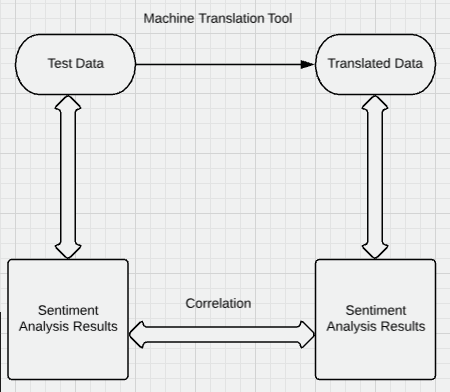
\includegraphics[width=.8\linewidth]{./img/testingModel.png}%
          }
          \medskip
  \end{minipage}
When we testing Machine Translation. We need assuming sentiment analysis tools
are profect correct. We can compare correlation coefficient between both side of
sentiment analysis results for getting which machine translation are better.
There is an example for testing Chinese to English machine translation.
\begin{enumerate}
  \item Using Google, Baidu, Yandex translation tools, translated original Chinese data to English data
  \item Using same sentiment analysis tool analysis original chinese dataset and
    translated dataset
  \item Calculate correlation coefficient between Chinese sentiment analysis
    results and English sentiment analysis results
  \item Compare correlation coefficient values. if value is bigger than others,
    we can say this translation tool, which use in original dataset to English
    dataset, can achieve better results than others.
  \end{enumerate}
For testing sentiment analysis tools, we can using same model. We need assuming
Machine Translation tools are profect correct. If right side of sentiment
analysis result is opposite attitude with left side of sentiment analysis
result. We can say we are detected one failure.
\item {Finding the best compound mode for machine translation service and
    sentiment analysis services} \\
  In this part, we totally have 6 kinds of compound model, which are Google
  translation with Google sentiment analysis; Yandex translation with Google
  sentiment analysis; Baidu translation with Google sentiment analysis; Google
  translation with Baidu sentiment analysis; Yandex translation with Baidu
  sentiment analysis and Baidu translation with Baidu sentiment analysis. we can
  using mean-square error (MSE) and Receiver operating characteristic (ROC)
  compare with user rate get the best compound model.
\item {Create own sentiment analysis model} \\
  Accounting to Liu said, creating sentiment analysis model have five steps. I will basis
  on this five steps for create my own model \cite{liu2012survey}.
  \begin{enumerate}
    \item{GetTerms - Reduce review to the list of keywords}
    \item{Filtering - Remove unnecessary keywords that will not add value for
        sentiment analysis, such as is, but, it etc}
    \item{Find the Base Word - Convert all inflections to their root word}
    \item{Make Features - Use the root words as features to indicate the
        positiveness or negativeness}
    \item{Classifier - Train a classifier to predict positivity}

  \end{enumerate}
\end{enumerate}
\paragraph{Implications or significance of the problem}
Social Media has been becoming more and more widely used. Accounting to Perrin's
survey, there are only $7\%$ American adults are use social media in 2005.
However, social media usage increase rapily, there are $65\%$ American adults are use
social media untill 2015 \cite{perrin2015social}. In our survey, we also find most of people
are insterest in different language speakers' opinions and attitudes. In
addition,
Most people enounter language and cultureal barriers during cross-language
communication.
As Dr. Haiyun mentions, English language sentiment analysis research has
undergone major developments in recent years \cite{ChineseSentimentAnalysis}.
However, less research has been undertaken in other languages, such as Chinese.
Today, a lot of English language sentiment analysis theories have been
developed. Also, a variety of Machine Translation tools is available, such as Google
translation, Bing translation and Yandex translation.
Manchine Translation uses computational linguistic programs and natural language
processing theory \cite{machineTranslation}.
However, nobody working in a combination of these two fields of research has undertaken non-English
sentiment analysis. Therefore, the research described and discussed in this paper aims to create a testing model to find the best-combination of English
sentiment analysis tools and machine translation tools to obtain reliable
sentiment analysis results from non-English texts, for non-English speakers who
do not have such sentiment analysis tools to analyze their own language.
Eventually, everyone will be able to understand different language speakers'
attitudes (positive or negative), emotions and opinions.\\
\paragraph{Expected Outcomes}

\section{Survey - Questionnaire}\label{survey}

Link : \hyperlink{https://www.surveymonkey.com/r/GHBDPBL}{https://www.surveymonkey.com/r/GHBDPBL}


\paragraph{}
The following questionnaire on Survey Monkey composed of 10 questions is used for our research work :

\begin{enumerate}
    \setlength\itemsep{1em}
    \item What is your gender ?
    \begin{enumerate}
        \item Male
        \item Female
        \item Other
    \end{enumerate}
    \textit{Initial Code : Gender}

    \item What are your areas of interest ? (many answers possible)
    \begin{enumerate}
        \item Sport
        \item Music
        \item Watching Videos / Films
        \item Reading
        \item Cooking
        \item Doing Shopping
        \item Chatting
        \item Playing Video Games
        \item Other (please specify)
    \end{enumerate}
    \textit{Initial Code : Interest areas}

    \item How often do you use social media ?
    \begin{enumerate}
        \item Always
        \item Usually
        \item Sometimes
        \item Rarely
        \item Never
    \end{enumerate}
    \textit{Initial Code : Frequency of social media use}

    \item Which social media do you use regularly ? (many answers possible)
    \begin{enumerate}
        \item Facebook
        \item Twitter
        \item YouTube
        \item Instagram
        \item WeChat
        \item LinkedIn
        \item Weibo
        \item I don't use social media
        \item Other (please specify)
    \end{enumerate}
    \textit{Initial Code : Types of social media}
    \item Which language(s) can you read ?
    \begin{enumerate}
        \item English
        \item French
        \item Chinese
        \item Spanish
        \item Vietnamese
        \item Arabic
        \item Indian
        \item Russian
        \item German
        \item Other (please specify)
    \end{enumerate}
    \textit{Initial Code : Language skills}

    \item Are you interested in other cultures ?
    \begin{enumerate}
        \item Extremely interested
        \item Very interested
        \item Somewhat interested
        \item Not so interested
        \item Not at all interested
    \end{enumerate}
    \textit{Initial Code : Attitude towards culture}

    \item Are you willing to try to understand a comment in an unknown language ?
    \begin{enumerate}
        \item Very likely
        \item Likely
        \item Neither likely nor likely
        \item Unlikely
        \item Very unlikely
    \end{enumerate}
    \textit{Initial Code : Behavior towards unknown languages}
       \item How often do you read others' opinion in social media posts ?
    \begin{enumerate}
        \item Always
        \item Usually
        \item Sometimes
        \item Rarely
        \item Never
    \end{enumerate}
    \textit{Initial Code : Interest in others' opinion}

    \item Which machine translation tool do you mostly use ?
    \begin{enumerate}
        \item Google Translation
        \item Microsoft Bing Translation
        \item Yandex Translation
        \item Baidu Translation
        \item Youdao Translation
        \item Other (please specify)
    \end{enumerate}
    \textit{Initial Code : Types of translation tools}

    \item Sentiment analysis tool can determine the attitude (positive or negative) of writers, which can be useful for analyzing a huge amount of comments. Are you willing to use this tool for analyzing your interest topic in social media, such as product comments or restaurant review, etc?
    \begin{enumerate}
        \item Very likely
        \item Likely
        \item Neither likely nor likely
        \item Unlikely
        \item Very unlikely
    \end{enumerate}
    \textit{Initial Code : Attitude towards sentiment analysis}

\end{enumerate}

\bibliographystyle{IEEEtran}
\bibliography{library}
\end{document}
